\documentclass[a4paper, 12pt]{article}

\usepackage{natbib}
\usepackage{amsmath}
\usepackage{amssymb}
\usepackage{amsfonts}
%\usepackage{graphicx}
%\usepackage[outdir=./]{epstopdf}
%\usepackage{notoccite}
\usepackage{graphicx}
% Expectation symbol
\DeclareMathOperator*{\E}{\mathbb{E}}

\begin{document}





\section{Introduction}

This paper presents an algorithm for surface classification using millimeter-wave radar. 

Fundamentally, radar is based on the concept of transmitting and recieving electromagnetic radiation. Radar response depends on the surrounding region of the sensor as objects in its vicinity scatter transmitted waves differently \citep{richards_2014}.  

 As technolgy is becoming increasingly intertwined with everyday life a multitude of new areas for smart sensing has opened up. One sensor category that has been recieving much attention is radars with very high frequency. These sensors combine a multitude of desirable features packed into a favorable form factor. These capabilities has made high frequency radars an increasingly popular choice in a steadily growing number of applications, such as monitoring of vital signs \citep{kuo_lin_yu_lo_lyu_chou_chuang_2016}, gesture recognition \citep{lien_gillian_karagozler_amihood_schwesig_olson_raja_poupyrev_2016}

Alongside with this development another trend within data science has emerged; the movement towards machine learning centric methods . This transition, spanned over multiple decades, has placed machine learning as one of the main-stays of information technology and a rather central part of our life. With ever increasing amounts of data, smart data analysis has proven key for technological progress \citep{a_smola_svn_vishwanathan_2010}.

Machine learning algorithms fundamentally utilizes various statistical techniques in order to allow computer systems to progressively improve performance. Data scientists have found this subclass of aritficial intelligence extremely practical, especially for data that lack an easily predictable structure. 

The amount of millimetre-wave radar applications is growing steadily.

With a continuously increasing demand for small sensors for use in a world where 

\subsection{Motivation}

Classification of surfaces is an important task. It appears in many areas.
\\ \\
You can determine surfaces in many different ways - optical, probing etc.
\\ \\
\noindent Optical: Images has been successful in determining surface roughness. One such method involves images of three-dimensional surface textures under different directions of illumination, and after some image processing techniques using a support vector machine for classification \citep{dong_duan_yang_2008}. 
\\ \\
\noindent Probing: One may also measure directly onto a surface directly through a probing approach. By sweeping a thin film across a fabric with constant contact force a depth-dependant charge is induced. After reading the output charge over some time interval it is then possible to extract information for detecting the texture of the fabric \citep{song_han_hu_li_2014}. A similar approach was used in \citep{strese_schuwerk_iepure_steinbach_2017}, where again surface classification was performed through direct contact. In this case features where instead extracted from the sound produced by vibrations generated by the movement. 
\\ \\
It is often desirable to to this without direct contact i.e. probing
\\ \\
Localization is the classic use-case for radars. 
\\ \\
Radar classification: Previous work and how they are different: A major challenge in radar sensing is to not only detect, but also to identify radar targets. This can for example be used for monitoring of urban environments with digital beamforming \citep{harter_kowalewski_sit_jalilvand_ziroff_zwick_2014}, or with a radar system mounted on a rotary table unit. 

 of urban environments and automotive radar 
\\ \\
Applications involving millimetre-wave radars and surface recognition is scarce.  
\\ \\
These radars commonly have wavelenghts of something something
\\ \\
If we however want to classify surface materials using a much shorter wavelength, the task changes dramatically as apsorption is near-instant. 
\\ \\
Something about radar wavelenght categories
\\ \\
Furthermore, radar sensors are commonly used in an array setting which permits beamforming and extraction of spatial information. 
\\ \\
If one on the other hand only has a singular radar sensor this is not possible and you must resort to other means.
\\ \\
Probably want something about IQ demodulation somewhere in here.

\subsection{Problem formulation}

We develop a pipeline for effectively solving this problem. 
\\ \\
We present modelling options with high accuracy and efficacy. 
\\ \\ 
We present results based on a 60GHz Acconeer micro radar. 
\\ \\
In this paper we introduce means of surface identification based on the output from a single 60 GHz radar sensor moving across a surface with constant height. 

\subsection{Thesis outline}

In chapter 2 we present an overview of a general radar system and introduce some crucial concepts for understanding the radar output used in this work. In chapter 3 we proceed by presenting our measurement setup and comment on the data collecting process and the data itself. Chapter 4 revolves around discussing ways of preprocessing the data and extracting relevant features from it. After the preprocessing, in chapter 5, we go through different classification schemes we have tested. The classification results are presented in a table for easy comparison. Finally, we conclude with an overall discussion of the work in chapter 6 and summarize our conclusions in chapter 7.

%Chapter 3: Mention something about the data collecting process. Motive our choice of parameters such as sampling frequency. Go through visual observations of our data.

%Chapter 4: Feature selection and preprocessing is considered. Signal structure is discussed primarily on an intuitive level. 

%Chapter 5: Classification schemes. Moving from simple to advanced, some classifiers of special interest are investigated. Results with regards to these classifiers are presented.

%Chapter 6: Disucssion.

%Chapter 7: Conclusion.

\section{Chapter 2: Radar system overview}

In this chapter we introduce a few fundamental radar concepts which will be important for understanding the data acquired by the 60 GHz sensor.
\\ \\
The radar equation.
\\ \\
The matched filter.
\\ \\
The IQ demodulation scheme. 
\\ \\
The radar system used for this project is a 60 GHz radar developed by Acconeer AB.



\subsection{The radar principle}

The radar principle is at its core simple.  A wavelet pulse $x_T(t)$ with some carrier frequency $\Omega$  is transmitted towards an object of interest. After some short time $t_1$, the radar listens for an echo. If no echo is received, it means there is no object present at distance\footnote{The reason for dividing by 2 is that the wavelet pulse must first travel from the radar to the object, and then find its way back to the radar.}
\begin{equation}
	d_1 = \frac{v_0\cdot t_1}2
\end{equation}
where $v_0$ is the speed of an electromagnetic wave in air. After the previously transmitted wavelet is guaranteed to have died out, a new one is transmitted. Again, the radar listens for an echo, but this time after another time $t_2$ has passed. $t_2$ is greater than $t_1$, meaning the radar listens for echoes further away. If an echo is received, it means there is an object present at distance 
$
	d_2 = \frac12(v_0\cdot t_2).
$
This process is repeated for different time delays $t_i$. The chosen time delays can be adjusted depending on in what ranges one wants to search in, and how good range resolution one seeks.

Together, the echoes (or lack thereof) from each transmitted wavelet make up one sweep. A sweep is often plotted in an amplitude-vs-range, or amplitude-vs-depth diagram as in figure (...). This plot is a good way to visualize at what ranges objects are present.

* Plot of sweep *

\subsection{Elements of a pulsed radar}

A pulsed radar system can be realized in countless ways, but all subscribe to the fundamental physical laws of electromagnetic radiation previously described. In this section one such configuration for a pulsed radar system is described.

A waveform generator outputs a radar envelope which is modulated by a local oscillator to some desired radio frequency. After signal amplification the wavelet is transmitted through an antenna. 

Detection is performed by a second antenna, which receives the returning signal during some time interval. The received signal then goes through a process known as \emph{mixing}. An internal wavelet is generated at a very specific delay from the initial pulse transmission and multiplied with the received signal. If the received and internal pulses do not match, the output of this multiplication will be zero. If there however exist some overlap between the internal and returning signals the output will be nonzero, indicating some level of energy content at the distance corresponding to the internal pulse delay. By increasing the internal pulse delay and repeating this procedure a set of measurement points is obtained. Mixing is thus achieved by multiplying a large number of returning wavelets with internally generated wavelet counterparts, adding a slight delay between sampling points. 


\includegraphics[scale=0.5]{figs_temp/mixing0}

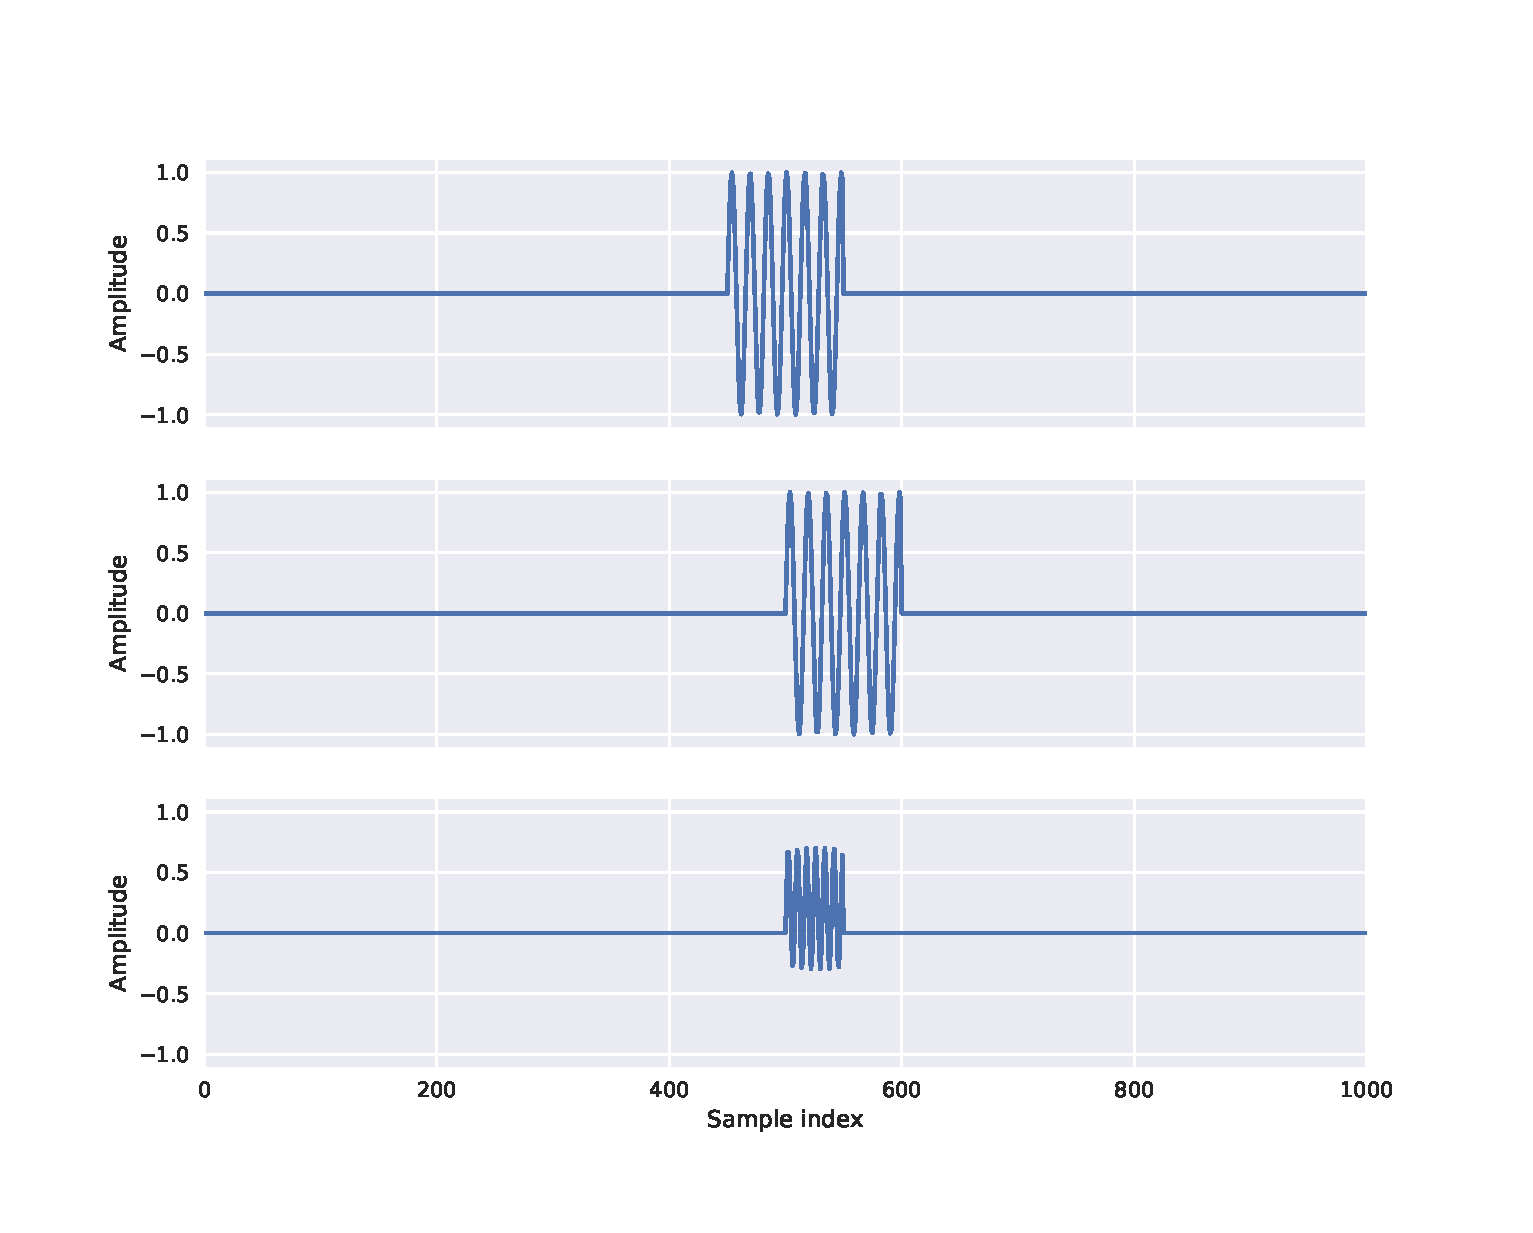
\includegraphics[scale=0.5]{figs_temp/mixing1}

\includegraphics[scale=0.5]{figs_temp/mixing2}




\subsection{IQ Data}
A common type of data when working with radar signal processing is in-phase and quadrature-phase data (IQ-data).  This type of data is useful in that it contains information not only about amplitude, but about the phase of the radar signal as well \citep{richards_2014}. IQ-data is represented as complex numbers, and a radar sweep consists of several such complex numbers - one for each investigated range. To obtain the amplitude plot, as the one in figure .... for a sweep, $s$, made up of IQ-data, one simply computes the absolute value for each complex number in $s$. Similarly, a phase curve can be obtained by computing the phase in each point. A phase curve can typically look like the one in *Figure of phase plot*

In many applications, the phase information in IQ-data is used when small changes in the radar signal need to be detected, (Mention a case such as recording over grass...) as the phase is more sensitive to changes than the amplitude \citep{lien_gillian_karagozler_amihood_schwesig_olson_raja_poupyrev_2016}. If an object is detected at distance $r(t_1)$ from the radar at time $t_1$, and shortly thereafter, the object is moved to distance $r(t_2)$, the corresponding difference in phase will be
\begin{equation}
	\label{eq:phase_diff}
	\Delta\phi(t_1, t_2)=\frac{4\pi}{\lambda}(r(t_2)-r(t_1)) \quad\quad \textrm{mod 2$\pi$}
\end{equation}
By having a sampling frequency which is too low, the range difference in $\eqref{eq:phase_diff}$ could potentially become very big, and the phase difference would fluctuate over time and be incomprehensible.

In the case of material classification, a high sampling frequency is highly beneficial. When moving across surfaces characterized by tiny details, a high sampling frequency is essential in capturing the shape of these.

For a thorough description of how IQ-data is derived from raw radar data, we refer to \citep{richards_2014}

\section{Data}
\subsection{Data Collecting}
Having reliable data is a fundamental requirement in building a good model. There are many parameters to consider in optimizing the data collecting process. However,  finding an optimal solution is often impossible as the combinations are endless, but putting some thought into every decision often proves worthwhile. Below, we motivate our choices of sensor placement as well as various parameters.

\subsubsection{Measurement Setup}


Include graphics of the sensor placement etc. and describe the setup briefly. Possibly mention the $\frac14\lambda$ gap between the sensor and RLM plastic.
\subsubsection{Measurement Settings}
Having reliable data is a fundamental requirement in building a good model. Hence, choosing suitable parameters such as sampling frequency, regions of interest and planning a good measurment setup are all crucial tasks. The sampling frequency is particularly important to consider when working with means that could potentially cause aliasing. One such case is the DFT \citep{lindgren_rootzeŽn_sandsten_2013}. If the sampling frequency is too low, we get aliasing etc. etc. 

In order to assure that aliasing is avoided, the maximal frequency component registered by the radar must be surpassed by half the sampling frequency
\begin{equation}
	f_{max} < \frac{f_s}{2}.
\end{equation}
The sampling frequency can be chosen accordingly, assuming the maximal frequency component is known. 

In figure (fig. from previous subsubsection) a vehicle is moving forward with constant speed, having a sensor mounted at the front. As it moves forward, small objects on the ground get closer to the radar sensor with some speed. This gives rise to a doppler frequency being registered by the radar, which is \citep{lien_gillian_karagozler_amihood_schwesig_olson_raja_poupyrev_2016}
\begin{equation}
	f_{d} = \frac{2v_\perp}{\lambda}.
\end{equation}
...


\subsection{Chapter 2.5: Data exploration}

Good source on PCA
\cite{hyvasrinen_karhunen_oja_2004}
PCA 125-143

Information theory
105-122
Argument for downsampling in range: In an information theoretic framework we interpret a random variable by how unpredicable or unstructured an observation of the variable is. This concept, examining the randomness of a variable, is commonly measured through entropy. Directly related to entropy is mutual information which essentially is how much information each member of a set have on the other members. \cite{hyvasrinen_karhunen_oja_2004}. Ideally one wants measurements that have a low measure of mutual information, meaning that each datapoint contain information not found elsewhere in the set. 

Observing a typical radar sweep[ref to plot with sweep] we note that points are very closely related on a small range scale, and nearly identical if we were to examine them on a sample by sample basis. One could argue that the mutual information found in the set is very high and that the entropy in each datapoint is low. Hence, to lower the first and increase the latter, one could downsample by some factor $D$ in range without significant loss of information.


PCA 125-143: Through the point and feature selection methods described in previous sections we obtain high dimensional feature vectors. Getting an intuitive feel for such data extracted in these processes is difficult as direct plotting is limited to three dimensions. 

Principal Component Analysis (PCA) is  a classical technique in statistical data analysis which takes a large set of multivariate variables and finds a smaller set of variables with less redundancy. Critically, PCA finds a rotated orthogonal coordinate system such that the elements of the set become uncorrelated. Projecting elements on the principal axes corresponding to the directions of maximal variance a good approximation of the original data in lower dimension is obtained \citep{hyvasrinen_karhunen_oja_2004}. 

\section{Chapter 3: Feature selection}

In order to create an effective predictive model one must first select a set of features used to produce each classification. Both a science and an art, this process involves intuition, theory and a hefty amount of trial-and-error. Although a seemingly daunting task, for a model to be effective the feature selection procedure is key, and a carefully considered selection often generates significantly better results than one hastily put together. 

Ideally, one seeks a small set of variables which accurately captures the information content in a larger set of data. After reducing the number of features into a more manageable format it is then possible to obtain good results with significantly less computational load than if no feature selection had been considered. Furthermore, the feature selection process allows us to pinpoint what data characteristics we wish to monitor, and subsequently which data characteristics we can disregard. 

\subsection{Desirable traits}

In the present case the objective is to capture defining characteristics of a surface using one dimensional data obtained from a radar sensor placed some small distance above the surface of interest. Furthermore, the sensor is moving along some direction parallell to the surface plane, thus continuously altering the sensors surroundings. One may split up the possible methods of characterizing this data obtained through this process into two main categories: Methods which aim at capturing the overall spatial signal form, and methods which examine the temporal changes in radar response. 

The first of the two is straight forward; if the scattering surface can be assumed to maintain some defining characteristics at any given point time one could simply extract features relating to these characteristics to generate a classification. Say for example we are presented two surfaces with equivalent reflective properties but where one is rough and the other is smooth. For the smooth surface the scatterers behave more predictably than the rugged surface. This would mean that the main portion of scattered electromagnetic waves will scatter at the

one would expect to receive a strong response from a electromagnetic pulse sent at a zero degree angle of incidence. If one instead sends a pulse at a higher angle of incidence, one would expect the opposite as the scatterers of the smooth surface would primarily scatter away from the sensor yielding a weak response. For the rough surface on the other hand, scatterers direct an incoming reflection in a wider array of angles. 

% Fortsätt här


due to the various properties of the scattering surface in the vicinity 

we begin this section with a discussion 



In order to make sense of data one must impose some reasonable assumptions. 
\\ 
One idea is to view each measurement, taken at time instance $t$ at range $r$ for material $m$, as drawn from some 
complex distribution specific for that combination of $r$ and $s$ but independent of time of sampling $t$. 
\\
Yada yada there is two combatting ideas here

\subsection{Preprocessing}

\subsubsection{Downsampling}
Add reference to Information Theoretic part

Since the correlation between neighboring range samples is very high we can downsample without significant loss of information. The downsampling process essentially requires three hyperparameters: A starting range $R_{start}$ and an end range $R_{end}$ where we begin and end our downsampling process respectively, as well as a downsampling factor $D$.

\begin{equation}
	x_D(n, t) = x(R_{start} + nD, t) \quad \text{for}\quad n=0...\frac{R_{end}-R_{start}}{D}
\end{equation}

\subsubsection{Sweep Normalization}
The gain sensitivity of the Acconeer radar chips can vary a lot from sensor to sensor. Makes it meaningless to measure, and classify on one sensor which is very different from the one that measured the training data. 

Explain normalization procedure: divide all sweeps within a feature box with the total energy within that feature box. 

Mention this was the best approach, but do not go into detail about the other methods - if so, just mention them briefly.



\subsubsection{Using multiple sweeps for feature selection}

In the radar system multiple sources of noise are introduced.
\\ \\
Noise sources: Thermal emissions of target, random currents in electrical components, data quantization, etc. etc. \citep{w_doerry_2016}
\\ \\
In the beginning section of this chapter we introduced two conflicting interpretations of the radar signal. In the first the incomming wavelet is drawn from a complex distribution, and each sweep is independent from the rest. In the second we instead considered that there may be some significant correlations in time to take into account; surface shapes and objects passing by the sensor are detected multiple times in a perhaps predictable and useful manner.  

The first suggest that signal averaging over a number of sweeps should yield a more and more accurate estimate. Thus the first approach greatly benefit from using multiple sweeps to find an average over some predefined number of sweeps.  In order to utilize the time correlations assumed in the second interpretation processing in time is of course demanded, and a number of sweeps need to be analyzed at once to extract features related to this way of viewing the radar response. 

Thus a predefined number is chosen as the number of sweeps used to extract each feature. While each feature may be extracted with higher accuracy, it is done at the price of a lower number of classifications per second. The relation between classification rate $F_c$, sampling speed $F_s$ and sweeps per feature $T_s$ is



\begin{equation}
	F_c = \frac{F_s}{T_s}
\end{equation}

\subsection{Features}

Fast time and slow time features 



\subsubsection{Expected signal}
The simplest way of selecting features would be to use plain sweep data as features. While this method requires very little data preprocessing, it does not give very good results (Any comment on how well it performs?). With just a little more effort, a significant improvement can be made by averaging a few sweeps in slow time, making the samples more similar. For range bin $i$, $T$ consecutive samples in slow time are collapsed into one according to

\begin{equation}
	s_i(t_m) = \E\{X_{i,t_m}\} = \frac{1}{T}\sum_{t=0}^{T-1}x(i, t_m + t)
\end{equation}

Figures: Sweep averaging plot (?), comparing averaged sweeps for different materials

\subsubsection{Average energy}
The average energy in a sweep tells us how much energy is reflected back to the radar. Hence it can be regarded as a measure of how good of a reflector the underlying surface is. The energy depends on the shape of the surface, as well as its dielectric constant. Compared to other materials, grass has a very different surface shape, which potentially gives it a very different reflexivity. However, its dielectric constant could also vary a lot depending on whether it is wet or dry, making it hard to guess its reflective properties.

By computing the average energy of single sweeps from different surfaces we obtain the results in figure (plots of sweep energies). Clearly, the grass surface has a much lower energy. $<$We have to compare different types of grass. Wet, dry, tall, short, etc.$>$

To get a more robust measure of the average energy we not only compute the average over selected range bins of a single sweep, but we average over a few consecutive sweeps as well. Mathematically, the feature we end up using becomes
\begin{equation}
	P(t_m) = \frac{1}{NT}\sum_{t=0}^{T-1}\sum_{n=0}^{K-1}x(n, t_m + t)x^*(n, t_m + t).
\end{equation}
Add some talk about this feature being left unused due to normalization.



\subsubsection{Fourier Transform}
A "feature box" consisting of $T$ sweeps is selected. Viewing this as a matrix with elements $X_{n,t}$, where $n$ denotes slow time, and $t$ fast time we can write a Fourier transform in slow time at range $r$, within this box as
\begin{equation}
	\mathbb{X}_k^{(r)} = \sum_{n=0}^{T-1}X_{n,r}\exp\Big[-2\pi i\frac{nk}{T}\Big] \quad k=0, ..., T-1
\end{equation}
To avoid aliasing we refer to chapter earlier in report where this is discussed. Mention that $\mathbb{X}_k^{(r)}$, for all $r$, $k$, is flattened to a vector, resulting in one new sample.




\subsubsection{Variance}

Include a discussion about the biased/unbiased estimate \\

Assume $x(n,t)$ are samples from a complex normal distribution $X_{n,t}$. Variance $v_i(t_m)$ at range $i$ at time $t_m$ can then be approximated using

\begin{equation}
\label{eq:var}
\begin{gathered}
	v_i(t_m) = \E\{ (X_{i,t_m} - \E\{X_{i,t_m}\})^2\} \\
	= \frac{1}{T-1}\sum_{t=0}^{T-1}(x(i, t_m + t) - s_i(t_m))^*(x(i, t_m + t) -  s_i(t_m))
\end{gathered}
\end{equation}

\subsubsection{Autocovariance in slow time}

\textbf{Add some motivation for using autocovariance}

\noindent
For some stochastic process $P_t$ we can define the autocovariance $\gamma$ as

\begin{equation}
	\gamma(t, s) = \E\big\{(P_t - \mu_t)(P_s - \mu_s)\big\}
\end{equation}

If $X_t$ is a weakly stationary process the first moment (mean) and autocovariance do not vary over time.  The autocovariance then only depends on the difference between $s$ and $t$, making it possible to rewrite as

\begin{equation}
	\gamma(\tau) = \E\big\{(P_t - \mu)(P_{t+\tau} - \mu)\big\}
\end{equation}

Assuming weak stationarity over a few rangebins we can estimate the autocovariance in slow time for each selected range. 

\begin{equation}
\begin{gathered}
	\gamma_i(t_m, \tau) = \E\big\{(X_{i,t_m} - \E\{X_{i, t_m}\})^*(X_{i, t_m+\tau} - \E\{X_{i, t_m+\tau}\})\big\}\\
	= \frac{1}{T-1}\sum_{t=0}^{T-1-\tau}(x(i, t_m + t) - s_i(t_m))^*(x(i, t_m + t + \tau) - s_i(t_m + \tau))
\end{gathered}
\end{equation}•

We can drop the $\tau$ in the final expectation term, as $s_i(t)$ are estimated in batch from $t_m$ to  $t_m + T$ yielding

\begin{equation}
	\gamma_i(t_m, \tau) = \frac{1}{T-1}\sum_{t=0}^{T-1- \tau}(x(i, t_m + t) - s_i(t_m))^*(x(i, t_m + t + \tau) - s_i(t_m))
\end{equation}
as our expression for autocovariance. Note that the variance in \ref{eq:var} collapses to the autocovariance at 0 lag. 


\section{Chapter 4: Classification schemes}

\subsection{LSTM}
Observing one range bin at a time, one could think of the radar data as a time series. This motivates the use of some classification scheme that exploits temporal behaviour. Recurrent neral networks (RNNs) feature this by having feedback within individual layers in the network. \citep{karim_majumdar_darabi_chen_2018} The problem with RNNs, however, is that they suffer from a vanishing or exploding gradient, and can only sustain a short term memory. A way to combat this is to use a neural network layer called long short term memory (LSTM). These are thoroughly described in, for example \citep{hochreiter_schmidhuber_1997}

LSTM-layers have previously been used successfully for classifications in radar applications. For instance in \citep{jithesh_sagayaraj_srinivasa_2018} the method was able to classify flying objects from $\textbf{nnn}$ different classes with an accuracy of ...? In \citep{karim_majumdar_darabi_chen_2018}, the LSTM layer is used in combination with a fully convolutional neural network (FCN), which proves to be a significant improvement from just using FCNs when classifying time series.

\section{Chapter 5: Discussion}


\subsection{Moisture}

One particularly challenging aspect of adequately classifying surfaces is the ever-changing environmental conditions surronding the sensor. Of particular interest is the moisture content in the surfaces of interest. Greater soil moisture implies higher dielectric constant, which in turn increases radar wave scattering \citep{rappaport_2006}. Thus a single surface may very well change its scattering properties over time. 

% More things that make selecting data tricky

\subsection{Surface variances}

Such effects is difficult to account for when selecting data. Gather a dataset as diverse as possible

\subsection{Individual sensor performance}
Despite the fact that the radar sensors have high precision, the output can vary a lot from sensor to sensor. In particular, one sensor can have a significantly higher gain than another, meaning that two sensors can have a different measure of reflexivity on the very same surface. This problem can be dealt with in several ways. 

Mention what we did, and discuss pros and cons.

1. Choose features that are not affected by the issue. Normalize sweeps etc.
	A. Normalize sweeps so that the main peak is at height 1
	B. Normalize sweeps by dividing with mean 

\newpage
\bibliography{refs}
\bibliographystyle{apalike}


\end{document}
